\chapter{Methodology and System Design}
\label{chap:methodology}

This chapter explains the main research steps followed in the project and the
design of the final system. It covers how the data were prepared, how the
classifiers and GANs were trained, how synthetic URLs were selected, and how
the models were evaluated and deployed. Its purpose is to make the experimental
procedure clear and reproducible; individual source-code functions and
programming instructions are outside the scope of this chapter.

\section{Research Design}

The project used an experimental comparison design. A phishing URL was treated
as the positive class and a legitimate URL as the negative class. The main
question was whether adding GAN-generated phishing URLs to a fixed real
training set changed detection performance on data that was not used for
training or model selection.

The central comparison was therefore
\begin{equation}
    \text{fixed real training data}
    \quad\text{against}\quad
    \text{the same real data plus synthetic phishing URLs}.
    \label{eq:method-main-comparison}
\end{equation}
The validation and test sets, model family, random seeds, preprocessing,
threshold rule, and evaluation metrics were held fixed within each controlled
experiment. A synthetic condition was not changed simply because it failed to
beat the real-only control. No improvement, or a small reduction, was retained
as a valid result.

The work used three levels of evidence:

\begin{enumerate}
    \item \textbf{Internal evaluation} measured performance on a frozen,
    hostname-separated test drawn from the same main source as training.

    \item \textbf{External evaluation} measured transfer to separately
    collected legitimate and phishing URLs with no accepted identity overlap.

    \item \textbf{Browser evaluation} tested the exported model, decision
    policy, inference reliability, and voluntary user feedback in the working
    extension.
\end{enumerate}

The design deliberately separates these levels. High internal performance does
not by itself prove that a model transfers to a new URL source, and a working
browser interface does not by itself prove production readiness.

\begin{figure}[htbp]
\centering
\setlength{\fboxsep}{7pt}
\fbox{\parbox{0.82\textwidth}{\centering
\textbf{Collect and freeze real URL data}\\
source labels, hashes, class counts, and permitted use}}

\vspace{0.35em}
$\Downarrow$
\vspace{0.35em}

\fbox{\parbox{0.82\textwidth}{\centering
\textbf{Normalize, deduplicate, and split by hostname}\\
training, validation, calibration, internal test, and external test remain separate}}

\vspace{0.35em}
$\Downarrow$
\vspace{0.35em}

\fbox{\parbox{0.82\textwidth}{\centering
\textbf{Train real-only classifiers and phishing URL generators}\\
same registered training identities; generator receives phishing training rows only}}

\vspace{0.35em}
$\Downarrow$
\vspace{0.35em}

\fbox{\parbox{0.82\textwidth}{\centering
\textbf{Filter and freeze synthetic pools}\\
validity, uniqueness, real overlap, structure, diversity, and challenge checks}}

\vspace{0.35em}
$\Downarrow$
\vspace{0.35em}

\fbox{\parbox{0.82\textwidth}{\centering
\textbf{Train controlled real-only and augmented conditions}\\
same architectures, seeds, validation sets, thresholds, and test sets}}

\vspace{0.35em}
$\Downarrow$
\vspace{0.35em}

\fbox{\parbox{0.82\textwidth}{\centering
\textbf{Evaluate, calibrate, export, and test in the browser}\\
internal, external, low-prevalence, challenge, reliability, and user evaluation}}
\caption{Overall experimental workflow.}
\label{fig:method-workflow}
\end{figure}

\section{Development Through Three Versions}

The final methodology was reached through three project versions. These
versions are not treated as interchangeable repetitions because their datasets
and controls differ. They document how the research problem became more
precise.

\begin{table}[htbp]
\centering
\caption{Purpose of the three project versions.}
\label{tab:method-versions}
\small
\begin{tabular}{@{}p{0.10\textwidth}p{0.37\textwidth}p{0.43\textwidth}@{}}
\toprule
Version & Main purpose & Methodological lesson \\
\midrule
1 & Build the first complete baseline, GAN, augmentation, and outside-testing pipeline using the large original URL dataset. & Strong internal results and unique generator outputs were insufficient evidence of external transfer. \\
2 & Use one frozen real dataset for controlled real-only and 10--40\% augmentation comparisons across seeds. & Synthetic difficulty and diversity had to be studied separately from real-test accuracy; source shift remained a major problem. \\
3 & Diagnose source shift, introduce multi-source real coverage, train the hybrid system, improve the GAN design, calibrate thresholds, and export the browser model. & Fair data access, source-aware validation, low-prevalence testing, and deployment policy were as important as the classifier architecture. \\
\bottomrule
\end{tabular}
\end{table}

Version~1 established the initial working system, including the baseline
classifiers, GAN generators, and augmentation experiments. Its results
confirmed that the proposed approach could be implemented, while also showing
the need for more controlled experiments and external evaluation. Version~2 is
retained as the large controlled one-dataset study. Version~3 supplies the final
system and the main deployment-oriented evaluation. Earlier results are
reported with their original conditions and are not merged into a single
statistical average.

\section{Data Sources and Dataset Roles}

\subsection{Source separation}

The project uses legitimate and phishing URLs from more than one source. Each
source is assigned a stated role: training, validation, calibration, internal
testing, external testing, or browser-user evaluation. A URL collected for a
final test is not moved into training after its result is inspected.

The original Version~3 master file, \texttt{URLs\_New.csv}, contained 450,176
input rows. Cleaning and hostname-separated partitioning produced the frozen
original splits in Table~\ref{tab:method-v3-splits}. The generator contract
allowed only the 82,219 phishing URLs in the training split. Validation and
test phishing URLs were never supplied to a generator.

\begin{table}[htbp]
\centering
\caption{Frozen original Version 3 splits.}
\label{tab:method-v3-splits}
\begin{tabular}{@{}lrrr@{}}
\toprule
Split & Legitimate & Phishing & Total \\
\midrule
Training   & 276,400 & 82,219 & 358,619 \\
Validation & 29,535  & 9,948  & 39,483 \\
Internal test & 38,908 & 10,321 & 49,229 \\
\bottomrule
\end{tabular}
\end{table}

External transfer analysis later produced a multi-source stored training pool
of 363,692 real URLs. It contained 276,400 original legitimate URLs, 3,012
outside legitimate coverage URLs, 82,219 original phishing URLs, 2,000
PhishTank URLs, and 61 OpenPhish URLs. Identities previously frozen for external
evaluation were excluded from the added training material.

The initial SeqGAN study used the 82,219 original phishing training rows,
whereas MS-HardGAN-C used all 84,280 phishing rows in the multi-source pool.
This difference was appropriate for their original development stages, but it
could confound a direct comparison between the two generators. A later matched
generator experiment therefore retrained SeqGAN using the exact 84,280-row
phishing token file used by MS-HardGAN-C. File hashes confirmed byte-for-byte
identity. Each generator retained its registered architecture and training
objective; the downstream comparison then used the same 363,692 real HYB-MS
rows, 40,410 generated rows, three classifier seeds, calibration data, and
frozen tests. This experiment compares complete generator designs while
controlling their real phishing input.

A final registered update added 1,746 legitimate and 1,746 phishing URLs to
both final training conditions. Consequently, the final real-only file had
367,184 real URLs. The final browser candidate added 40,410 accepted synthetic
phishing URLs, producing 407,594 stored training rows. The two conditions
therefore differed only by the synthetic component.

\begin{table}[htbp]
\centering
\caption{Principal datasets and their permitted roles.}
\label{tab:method-dataset-roles}
\small
\begin{tabular}{@{}p{0.31\textwidth}rrrp{0.22\textwidth}@{}}
\toprule
Dataset stage & Legit. & Real phish. & Synthetic & Role \\
\midrule
Original V3 training & 276,400 & 82,219 & 0 & Baselines and generator input \\
Original V3 validation & 29,535 & 9,948 & 0 & Early stopping and initial thresholds \\
Original V3 internal test & 38,908 & 10,321 & 0 & Frozen internal evaluation \\
Multi-source real pool & 279,412 & 84,280 & 0 & MS and hybrid development \\
Matched generator input & 0 & 84,280 & 0 & SeqGAN/MS-HardGAN-C input control \\
Final updated real-only & 281,158 & 86,026 & 0 & Final real control \\
Final updated GAN condition & 281,158 & 86,026 & 40,410 & Final augmented model \\
Browser calibration cohort & 3,800 & 200 & 0 & Threshold selection only \\
Final browser test & 5,700 & 300 & 0 & Frozen low-prevalence test \\
Later external test & 9,700 & 300 & 0 & Post-freeze evaluation \\
\bottomrule
\end{tabular}
\end{table}

\subsection{Label convention}

The project uses $y=0$ for legitimate and $y=1$ for phishing. Incoming files
were not assumed to share this convention. Their labels were mapped explicitly
before concatenation. This was particularly important for
\texttt{new\_data\_urls.csv}, in which the source convention used 1 for
legitimate. Class counts were checked after every mapping so that a reversed
source could not silently enter training.

\subsection{Illustrative real URL records}

Table~\ref{tab:method-real-url-examples} gives a small set of records from the
stored project data. These examples are included only to make the two labels
concrete; they were not selected to demonstrate model performance. Phishing
addresses are defanged and identifying path tokens are shortened so that they
cannot be followed directly from the report. Their labels come from the stated
data source rather than from visual judgement by the author
\citep{phishtankdeveloper}.

\begin{table}[htbp]
\centering
\caption{Illustrative legitimate and phishing URL records used by the project.}
\label{tab:method-real-url-examples}
\small
\begin{tabular}{@{}p{0.16\textwidth}p{0.54\textwidth}p{0.20\textwidth}@{}}
\toprule
Label & Defanged or non-clickable example & Stored source and role \\
\midrule
Legitimate & \nolinkurl{https://www.google.com/} & \texttt{URLs\_New}; training \\
Legitimate & \nolinkurl{https://www.wikipedia.org/} & \texttt{URLs\_New}; training \\
Legitimate & \nolinkurl{https://ros.org/} & Tranco; external test \\
Phishing & \nolinkurl{hxxps://www[.]dpdlocoug[.]top/com} & PhishTank; external test \\
Phishing & \nolinkurl{hxxp://allegrolokalnie[.]lokalna-043289[.]shop} & PhishTank; external test \\
Phishing & \nolinkurl{hxxps://docs[.]google[.]com/forms/d/e/[redacted]/viewform} & PhishTank; external test \\
\bottomrule
\end{tabular}
\end{table}

\section{URL Preparation and Leakage Control}

\subsection{Normalization}

Each raw URL passed through the same deterministic preprocessing procedure. The
main operations were:

\begin{enumerate}
    \item remove surrounding whitespace and reject empty values;
    \item accept HTTP(S) URL structure and supply a parsing scheme when needed;
    \item normalize the hostname to lower case and remove user information;
    \item convert internationalized hostname components consistently;
    \item preserve meaningful path and query structure;
    \item remove the scheme from the model string; and
    \item produce one canonical string for duplicate and overlap checks.
\end{enumerate}

The scheme was removed after an audit showed that HTTP and HTTPS exposure could
act as a source shortcut. The model was intended to learn URL structure rather
than treat the presence of HTTPS as proof of legitimacy.

\subsection{Duplicate and conflict removal}

Duplicates were checked at several levels: raw normalized string, canonical
URL, encoded character sequence, hostname, and registered domain when
appropriate. Exact duplicates were removed. If the same canonical identity
appeared with conflicting labels, it was excluded from the controlled split and
recorded for inspection rather than being assigned an arbitrary class.

Generated URLs were also checked against all permitted real training rows. An
accepted synthetic pool could not contain exact duplicates, accepted real
overlap, or repeated generator templates above the frozen limit. These checks
distinguish novelty from simple memorisation.

\subsection{Hostname-separated splitting}

Random row splitting can place two paths from the same host in both training and
testing. The model may then recognise the host instead of learning transferable
phishing structure. To reduce this leakage, the main partitions were assigned
by hostname using a deterministic seed-42 hash. All URLs associated with one
hostname were placed in only one of training, validation, or test.

After splitting, automated assertions checked that the hostname intersections
were empty. Dataset counts and cryptographic hashes were stored with the
artifacts so rerunning a model could not silently use a different file.

\section{Input Representations}

\subsection{Character representation}

The neural sequence models use a 168-symbol vocabulary. Each standardized URL
is encoded as integer character identifiers and padded or truncated to 128
characters. An unknown-character symbol handles characters outside the fixed
vocabulary. Padding positions are excluded where the architecture supports
masking.

The 128-character limit keeps GPU memory and browser inference predictable.
Long URLs are not completely ignored by the hybrid because its lexical branch
still measures full URL, hostname, path, and query lengths. Nevertheless,
characters after position 128 are unavailable to the character branch and this
is treated as a stated limitation.

\subsection{Lexical representation}

The conventional RF and SVM experiments used URL-only lexical measurements.
The final hybrid used 35 scheme-neutral, Public-Suffix-List-aware features.
They covered:

\begin{itemize}
    \item total URL, hostname, registered-domain, subdomain, path, query, and
    fragment lengths;
    \item counts or ratios of digits, letters, dots, hyphens, slashes,
    underscores, percent signs, equal signs, ampersands, and other delimiters;
    \item subdomain depth, path depth, query parameter count, and hostname-token
    structure;
    \item IP-literal, punycode, port, and unusual-host indicators;
    \item character diversity and entropy-like measurements; and
    \item indicators for URL tokens commonly associated with account, login,
    verification, payment, or security wording.
\end{itemize}

Scaling statistics were fitted on training data only. Validation, calibration,
internal-test, and external-test rows did not influence the feature medians or
interquartile ranges.

\section{Classifier Design}

Five baseline families were retained because they represent different levels
of complexity. RF and linear SVM provide interpretable lexical references. RNN
and LSTM test sequential character learning. CNN tests local character-pattern
learning. The hybrid combines character and lexical evidence.

\begin{table}[htbp]
\centering
\caption{Classifier configurations used in Version 3.}
\label{tab:method-classifiers}
\small
\begin{tabular}{@{}p{0.16\textwidth}p{0.33\textwidth}p{0.40\textwidth}@{}}
\toprule
Model & Input & Main configuration \\
\midrule
RF & Lexical features & 300 trees, maximum depth 32, minimum leaf size 2, square-root feature sampling \\
Linear SVM & Scaled lexical features & $C=1.0$, maximum 20,000 optimisation iterations \\
RNN & Character sequence & 48-dimensional embedding, 96 hidden units, one tanh recurrent layer \\
LSTM & Character sequence & 48-dimensional embedding, 96 hidden units, gated recurrent representation \\
CNN & Character sequence & 48-dimensional embedding; 128 channels for kernels 3, 4, and 5; global maximum pooling \\
HYB-MS & Character sequence and 35 lexical features & CNN character branch, two-layer lexical branch, fused hidden layer, dropout, source-aware training \\
\bottomrule
\end{tabular}
\end{table}

\subsection{Fairness of classifier comparisons}

Fairness does not require every classifier to have the same architecture or
feature representation; that would remove the reason for comparing model
families. It requires that the compared conditions have equal access to the
registered real URL identities, use the same labels and evaluation rows, and do
not receive hidden test information.

Accordingly, models in each controlled comparison used the same permitted real
training rows. RF and SVM received the lexical representation suited to
traditional methods, while sequence models received characters. The hybrid's
use of both representations was declared as part of its architecture and was
compared against a real-only hybrid of identical architecture. In the fair GAN
experiment, the same accepted synthetic URL identities were supplied to every
classifier condition at the stated ratio.

\subsection{Hybrid multi-source model}

HYB-MS contains two branches. The character branch embeds the URL and applies
one-dimensional convolutional filters with widths 3, 4, and 5. Global maximum
pooling produces a fixed representation of local character patterns. The
lexical branch passes the 35 scaled features through two fully connected ReLU
layers. Both outputs are concatenated, passed through a fused hidden layer and
dropout, and mapped to one phishing logit.

\begin{figure}[htbp]
    \centering
    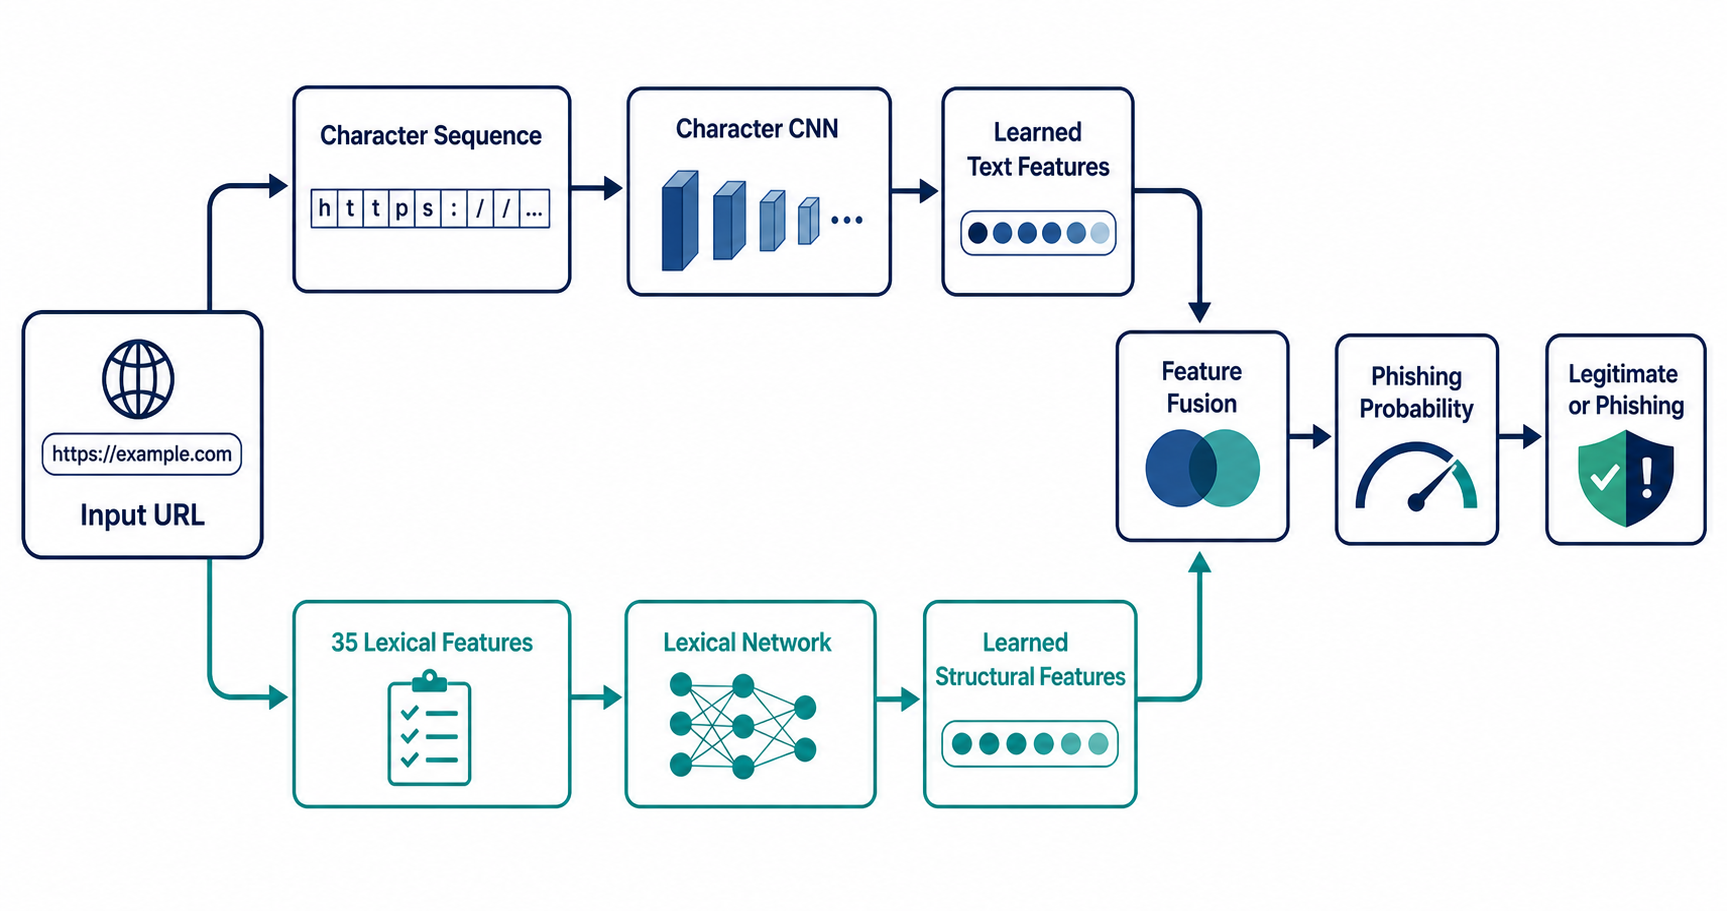
\includegraphics[width=0.96\textwidth]{figures/hybrid_architecture.png}
    \caption{High-level architecture of the hybrid URL classifier.}
    \label{fig:method-hybrid-architecture}
\end{figure}

The original HYB-MS training design also used weighted source sampling. The
363,692 stored real URLs remained unchanged, but sampling with replacement
controlled how often small outside sources were presented during an epoch.
This changed exposure frequency, not the number of unique stored URLs. Natural
sampling and weighted sampling are therefore reported as different conditions.

Class-conditional CORAL alignment was tested to reduce source-specific feature
differences. Legitimate representations were aligned only with legitimate
representations, and phishing representations only with phishing
representations. The registered CORAL weight was 0.01. This avoided forcing
opposite classes toward the same distribution.

\section{GAN Design and Training}

\subsection{Training corpus}

The initial Version~3 generators were trained on the 82,219 phishing URLs from
the original training split. Multi-source GAN development used 84,280 real
phishing URLs: 82,219 original URLs, 2,000 PhishTank URLs, and 61 OpenPhish
URLs. Generator validation and final classifier test rows were excluded.

Every text generator first learned next-character prediction by maximum
likelihood. Adversarial training followed only after this stage. This is needed
because direct adversarial learning over discrete characters is unstable;
SeqGAN addresses the problem through policy gradients \citep{yu2017seqgan},
while the other implemented text generators use a differentiable
Gumbel-Softmax approximation \citep{jang2017gumbel}.

\subsection{Implemented generators}

\begin{table}[htbp]
\centering
\caption{Implemented Version 3 GAN configurations.}
\label{tab:method-gans}
\small
\begin{tabular}{@{}p{0.15\textwidth}p{0.28\textwidth}p{0.27\textwidth}p{0.20\textwidth}@{}}
\toprule
GAN & Generator & Discriminator & Training schedule \\
\midrule
SeqGAN & Autoregressive character LSTM trained as a stochastic policy & Character CNN reward model & 5 MLE + 3 adversarial epochs; 100 adversarial steps/epoch \\
RelGAN & Relational-memory generator with four memory slots and four attention heads & Multi-representation character CNN & 5 MLE + 3 adversarial epochs; 150 adversarial steps/epoch \\
URL-GAN & Two-layer character LSTM with Gumbel-Softmax output & Character CNN with kernels 2, 3, 4, and 5 & 5 MLE + 4 adversarial epochs; 150 adversarial steps/epoch \\
MS-HardGAN-C & Conditional two-layer LSTM using structure, source, and latent inputs & Multi-head character CNN for authenticity, pattern, and source & 5 MLE + 4 adversarial epochs; 250 adversarial steps/epoch \\
\bottomrule
\end{tabular}
\end{table}

SeqGAN was retained because it is designed for discrete sequence generation.
RelGAN was implemented as a relational alternative, but its structural output
required particularly strict filtering. URL-GAN provided a simpler name and
architecture for the two-layer LSTM/CNN Gumbel design. MS-HardGAN-C was the
final source- and pattern-conditioned generator used to construct the
synthetic pool for the browser candidate.

\subsection{Classifier-challenging objective}

MS-HardGAN-C was designed to generate phishing-style strings that were not
merely easy copies of the training corpus. Frozen CNN, LSTM, and RNN
classifiers scored differentiable candidates. Their raw scores were first
converted to validation-based percentiles because the score scales of different
model families are not directly comparable. The mean challenge signal rewarded
candidates that multiple classifiers found difficult.

The challenge weight was 0.05 and began in adversarial epoch 3. It was evaluated
every fourth generator step. Realism, pattern classification, source
classification, maximum-likelihood regularisation, feature matching, and
diversity remained active. Thus, a malformed string could not succeed only by
receiving a low phishing score.

This procedure creates difficult stress examples based on known evidence. It
does not predict an unknown future attack concept. In the report these outputs
are described as challenging or zero-day-like samples, not as forecasts of
actual zero-day URLs.

\subsection{Epoch interpretation}

The final generator completed five full MLE epochs and four adversarial epochs
with 250 steps each, giving 1,000 adversarial update cycles. The neural
classifiers had a maximum of eight epochs and an early-stopping patience of two.
CNN, LSTM, and RNN baseline runs executed eight epochs, while the retained
checkpoint varied by seed.

The final augmented hybrid runs stopped after 3, 4, and 3 epochs for seeds 42,
43, and 44 and retained epochs 1, 2, and 1, respectively. Each epoch contained
hundreds of thousands of URL presentations. Stopping early therefore reflected
the registered validation rule rather than an attempt to reduce training work.
RF and SVM are not epoch-based: RF used 300 trees and SVM used iterative convex
optimisation with a maximum of 20,000 iterations.

\section{Synthetic URL Quality Control}

Generated data were evaluated before they were used for augmentation. The
quality procedure included:

\begin{enumerate}
    \item syntactic parsing and permitted-character checks;
    \item plausible hostname and top-level-domain-like structure;
    \item rejection of empty hosts, abnormal separators, repeated protocols,
    excessive padding, and other structural outliers;
    \item exact duplicate removal;
    \item exact and canonical overlap checks against real data;
    \item repeated-template and near-duplicate inspection;
    \item URL-length, token, path, query, and lexical-distribution comparison;
    \item uniqueness, acceptance, and memorisation measurements; and
    \item frozen-classifier challenge and held-out synthetic-challenge tests.
\end{enumerate}

\subsection{Illustrative generated samples}

Table~\ref{tab:method-gan-url-examples} shows compact examples taken from the
frozen MS-HardGAN-C 10\% pool. They are synthetic phishing candidates, not
confirmed live attacks and not predictions of future incidents. The displayed
strings are defanged; query values are shortened where necessary. They
illustrate the mixture of subdomains, path depth, digits, separators, and
unusual character sequences learned by the generator. These few examples are
for interpretation only; the quantitative quality measures were calculated on
the full accepted pool.

\begin{table}[htbp]
\centering
\caption{Illustrative defanged MS-HardGAN-C samples from the frozen 10\% pool.}
\label{tab:method-gan-url-examples}
\small
\begin{tabular}{@{}cp{0.78\textwidth}@{}}
\toprule
Pattern ID & Generated URL text \\
\midrule
0 & \nolinkurl{wwww[.]isfiontt0[.]com/wpatufin/tepeb/} \\
1 & \nolinkurl{wwwl[.]anferjalbi[.]cige[.]com/?eev=[redacted]} \\
2 & \nolinkurl{jilitebap[.]com/1/drrgg} \\
3 & \nolinkurl{ukuoll-seryin[.]com/wwfposidimatexej[.]cum/arinde/dalie[.]chl} \\
4 & \nolinkurl{megomlqr[.]com/wtuned/modir/ocoliraide/reglfinex20023[.]50} \\
7 & \nolinkurl{mlobacy[.]co/mlsrirud} \\
\bottomrule
\end{tabular}
\end{table}

Uniqueness alone was not treated as proof of quality. Random malformed strings
can be perfectly unique. The accepted pool therefore had to be novel, valid,
structurally plausible, sufficiently diverse, and free from permitted real-data
overlap.

The realism-filtered condition applied the frozen structural and lexical rules.
The realism-filtered plus challenging condition additionally preferred URLs
that several calibrated classifier families found difficult. Diversity caps
prevented selection from collapsing onto one generator, template, or lexical
cluster. Selection rules were frozen before final test labels were viewed.

\section{Augmentation Conditions}

Let $N_r$ be the number of fixed real training URLs and let $r$ be the desired
synthetic fraction of the final augmented dataset. The number of synthetic URLs
is
\begin{equation}
    N_g=\operatorname{round}\!\left(\frac{r}{1-r}N_r\right).
    \label{eq:method-augmentation-count}
\end{equation}
This definition means that a 10\% condition contains 10\% synthetic rows in the
combined file, rather than simply adding 10\% of the original row count.

\begin{table}[htbp]
\centering
\caption{Registered augmentation counts for the 363,692-row multi-source real pool.}
\label{tab:method-augmentation-counts}
\begin{tabular}{@{}rrr@{}}
\toprule
Synthetic fraction & Synthetic URLs & Combined rows \\
\midrule
10\% & 40,410 & 404,102 \\
20\% & 90,923 & 454,615 \\
30\% & 155,868 & 519,560 \\
40\% & 242,461 & 606,153 \\
\bottomrule
\end{tabular}
\end{table}

The synthetic pools were nested where possible so that a larger condition
extended the smaller pool rather than replacing it with an unrelated sample.
The real rows were preserved. Augmentation ratios were not changed after
observing test results to search for a winning configuration.

One additional controlled 10\% experiment compared four selection conditions:

\begin{enumerate}
    \item real-only;
    \item random accepted GAN augmentation;
    \item realism-filtered random augmentation; and
    \item realism-filtered plus classifier-challenging augmentation.
\end{enumerate}

All four conditions used the same real identities, synthetic count, seeds,
model settings, validation rows, thresholds, and test rows. Generator
composition was recorded so generator identity did not become a hidden
variable.

\section{Training and Model Selection}

Neural training used the NVIDIA RTX~3060 Laptop GPU, CUDA, mixed precision,
AdamW, gradient clipping, and deterministic seeds 42, 43, and 44. The maximum
classifier training length was eight epochs with early-stopping patience of two.
Class-weighted binary cross-entropy reduced the effect of class imbalance.

Checkpoints were selected using validation performance. For the source-aware
hybrid, the selection score combined the frozen original validation set and a
separate cross-source domain-validation set. This prevented a checkpoint from
being selected solely because it improved the familiar source while becoming
worse on the outside source.

Operating thresholds were selected on validation or calibration data. The
primary rule maximized the registered objective subject to the stated FPR cap.
The final test labels were not used to choose epochs, select synthetic samples,
calibrate the score threshold, or modify the browser decision tiers.

The three seed checkpoints were retained independently. For final ensemble
inference, their sigmoid scores were averaged:
\begin{equation}
    \bar p(u)=\frac{p_{42}(u)+p_{43}(u)+p_{44}(u)}{3}.
    \label{eq:method-ensemble}
\end{equation}
The browser uses the same three exported ONNX models. A parity test compared
PyTorch and ONNX outputs before the browser bundle was accepted.

\section{Evaluation Protocol}

\subsection{Classifier metrics}

The main labelled-dataset metrics were accuracy, precision, recall, F1-score,
ROC-AUC, FPR, and FNR. PR-AUC was also recorded where class imbalance made it
informative. Results across seeds were reported as mean and standard deviation,
and paired changes were calculated because the same seeds and test identities
were used in the compared conditions.

Accuracy was not treated as sufficient for deployment-like tests. When
legitimate URLs greatly outnumber phishing URLs, a small FPR can produce many
warnings, while a high FNR represents missed attacks. Therefore, low-prevalence
tests used both class-independent metrics and the resulting confusion matrix.

\subsection{Evaluation levels}

The following tests were kept separate:

\begin{itemize}
    \item the 49,229-row original internal test;
    \item identity-disjoint external sets, including frozen 10K, 20K, and 30K
    scenarios;
    \item later low-prevalence tests containing approximately 3--10\% phishing;
    \item long-legitimate-URL stress tests;
    \item PhishTank-focused phishing snapshots;
    \item frozen synthetic challenge sets not used to select augmentation; and
    \item browser ONNX parity, latency, duplicate-scan, and user tests.
\end{itemize}

The source and date of each external dataset were stored with its result. Test
identities were checked against training, calibration, and synthetic data before
metrics were calculated.

\subsection{DNS secondary experiment}

A separate experiment evaluated a real-data DNS classifier as secondary
evidence for uncertain URLs. It compared real-only and GAN-augmented primary
URL models while holding the DNS data and decision rule fixed. GANs generated
URL text only and did not create DNS observations.

The DNS experiment is supporting research rather than a feature silently added
to the browser model. The distributed extension uses the URL ensemble and its
local policy; this distinction is maintained in the implementation and results
chapters.

\subsection{Browser user-evaluation measures}

The browser exports do not contain independently verified labels for every
visited URL. Formal accuracy, precision, recall, F1, ROC-AUC, FPR, and FNR
therefore cannot be calculated from voluntary user feedback alone. Three
descriptive measures are used instead.

Let $N$ be unique evaluated URLs, $R$ be explicit false-alarm reports, and $A$
be caution, warning, or block decisions. The user-reported false-alarm rate is
\begin{equation}
    \mathrm{URFAR}=\frac{R}{N}\times100.
    \label{eq:method-urfar}
\end{equation}
The overall alert rate is
\begin{equation}
    \mathrm{OAR}=\frac{A}{N}\times100,
    \label{eq:method-oar}
\end{equation}
URFAR is a lower-bound descriptive rate unless the participant confirms that
all observed mistakes were reported. OAR measures warning burden and is not
called an FPR because some alerts may be correct. Feedback completeness is
recorded from direct participant confirmation; it is not estimated by dividing
reports by alerts, because feedback can be submitted from several decision
tiers. Labelled frozen datasets remain the source of formal classifier metrics.

\section{Browser System Design and Privacy}

The browser extension performs inference locally. The URL is canonicalized and
encoded using preprocessing resources packaged with the extension. Three ONNX
models produce scores, which are averaged and mapped to allow, secondary
review, caution, warning, or block tiers. Passive mode reports the decision
without navigation blocking; protection mode can display stronger warnings at
the frozen policy thresholds. Literal local and public IP addresses follow a
separate conservative rule because a domain-name model lacks normal hostname
context for them.

Repeated browser events can fire for the same navigation, history change, or
fragment. The user-evaluation build therefore deduplicates canonical URL
assessments and reports model executions separately from unique URL decisions.
This prevents repeated scans from inflating the study denominator.

Participation requires explicit local consent. Automatic raw URLs are not
uploaded or exported. Salted local fingerprints support deduplication, but the
fingerprints themselves are not included in the exported result. A URL is
stored in a feedback record only after the user deliberately reports a false
alarm or missed phishing case, and query values and fragments are removed from
that report. These controls reduce privacy risk while still permitting a small
usability evaluation.

\section{Reproducibility Controls}

The following controls were used throughout the final experiments:

\begin{itemize}
    \item configuration files store model dimensions, learning rates, epoch
    limits, seeds, augmentation ratios, and generator schedules;
    \item dataset and model files are identified by cryptographic hashes;
    \item training histories store each executed epoch and the retained epoch;
    \item checkpoints, predictions, thresholds, confusion matrices, and metric
    summaries are saved under versioned artifact directories;
    \item synthetic selection rules and accepted pools are frozen before final
    evaluation;
    \item internal, external, calibration, challenge, and browser results are
    stored separately; and
    \item earlier project versions remain archived instead of being overwritten
    by the final configuration.
\end{itemize}

These measures allow the final model to be reconstructed and prevent a good
result from depending on an undocumented dataset or threshold change.

\section{Chapter Summary}

The methodology uses a fixed-label URL classification problem, hostname-based
splits, explicit source roles, controlled real-only and GAN-augmented training,
three-seed evaluation, and validation-selected checkpoints and thresholds. The
final system combines a character CNN with 35 lexical features and uses a
three-seed ensemble. MS-HardGAN-C generates source- and pattern-conditioned
phishing URLs that must pass realism, novelty, diversity, and overlap checks
before augmentation.

Internal, external, low-prevalence, synthetic-challenge, DNS, and browser tests
are kept distinct. Formal classifier metrics are calculated only when verified
labels are available; browser feedback instead uses the reported-false-alarm
rate, overall alert rate, and participant-confirmed completeness status. The
next chapter describes the implemented system at a component level.
